%
% This file is part of Calicut University Question Paper Collection.
%
% Copyright (c) 2012-2015 Mohammed Sadik P. K. <sadiq (at) sadiqpk (d0t) org>.
% License: GNU GPLv3 or later
%
% Calicut University Question Paper Collection is free software: you can
% redistribute it and/or modify
% it under the terms of the GNU General Public License as published by
% the Free Software Foundation, either version 3 of the License, or
% (at your option) any later version.
% 
% Calicut University Question Paper Collection is distributed in the hope
% that it will be useful,
% but WITHOUT ANY WARRANTY; without even the implied warranty of
% MERCHANTABILITY or FITNESS FOR A PARTICULAR PURPOSE.  See the
% GNU General Public License for more details.
% 
% You should have received a copy of the GNU General Public License
% along with Calicut University Question Paper Collection.
% If not, see <http://www.gnu.org/licenses/>.
% 
%
\def \subj{AI 09 305---DIGITAL SYSTEMS}

\mainhead{D 51038}{2}
\semthree{NOVEMBER 2013}
\sub{\subj}
\maxtime

\partA

\iitem What is a parity bit? List its types.
\item Distinguish between PLAs and PALs.
\item State any \emph{two} advantages of CMOS Logic over other families.
\item State the difference between Mealy and Moore Machine.
\item What are the \emph{two} types of Asynchronous sequential circuits?

\markA
\partC

\item State and prove De Morgan's theorem.
\item Find the Canonical form of $f$(A, B, C, D) = ABC$'$ + AB$'$D + C$'$D
  + CD$'$.
\item Write a brief note on ROM.
\item Explain the operation of a JK flip-flop.
\item Explain the characteristics of ECL Logic.
\item What are cycles and races? How are they avoided?

\markB
\partC

\item \iitem Reduce the following expression using K-Map:

  $f$(A, B, C, D, E) = $\sum m(0, 2, 4, 15, 21, 27, 29) + \sum d (3, 5, 26)$.
\Or

\newpage \again

\item Minimize:

  F(A, B, C, D) = $\sum m(0, 1, 5, 7, 8, 9, 10, 11, 14, 15)$ using Quine
  McCluskey method.
\ene

\item \iitem Implement the following function using suitable multiplexers:

  F(A, B, C, D) = $\sum m(0, 2, 4, 6, 8, 10, 12, 14)$.
\Or
\item Implement a full adder using suitable decoder and additional logic
  gates.
\ene

\item \iitem Design a MOD-5 counter and explain its operation.
\Or
\item Explain the operation of a Monostable Multivibrator and astable
  Multivibrator.
\ene

\item \iitem Design a serial adder using Mealy state machine and explain
  its operation.
\Or
\item Minimize the state table give below:

\begin{flushleft}
  \hspace{1cm}\begin{tabular}{| c | c | c |}
  \hline
  {Present} & \multicolumn{2}{c|}{
  \rule{0ex}{2.5ex}Next state, Z (Output)}\\
  \cline{2-3}
   State & \multicolumn{2}{c|}{
  \rule{0ex}{2.5ex}X input}\\
  \hline
  & \ \ \ \ \ \ 0\ \ \ \ \ \ & 1 \\
  \hline
  A & B, 0 & C, 0 \\\hline
  B & B, 0 & D, 0 \\\hline
  C & B, 0 & C, 0 \\\hline
  D & E, 1 & C, 0 \\\hline
  E & B, 0 & D, 0 \\\hline
  
  \end{tabular}
\end{flushleft}
\ene

\markC
\ene

\newpage

\mainhead{D 30914}{2}
\semthree{OCTOBER 2012}
\sub{\subj}
\maxtime

\partA

\iitem Convert 22.20$_\text{10}$ to its binary equivalent.
\item Compare 1's complement and 2's complement form.
\item Design a Half Adder.
\item Convert JK flip flop into a D flip flop.
\item What is a totem pole output?

\markA
\partB

\item Write a note on Error detecting Codes.
\item State and prove De Morgan's theorem.
\item Simplify $\text{F} = \text{(A} + \bar{\text{B}} + \bar{\text{C}} \text{)}
 \text{(A} + \bar{\text{B}} + \text{C} \text{)}$.
\item Design a Binary-Gray decoder.
\item How frequency division is achieved using flip flops? Give the general expression
  for it.
\item State the condition for state equivalence Give an example.

\markB
\partC

\item \iitem Explain any one Error detecting and Correcting code.
\Or
\item Determine the prime implicants of the function.

  F(A, B, C, D) = $\sum (0, 1, 2, 3, 5, 6, 7, 8, 11, 13)$.
\ene

\newpage \again

\item \iitem Design an octal to binary encoder.
\Or
\item Discuss in detail about:
\iitem Static RAM.
\item Dynamic RAM.
\ene \ene

\item \iitem Design a 3-bit bidirectional shift register.
\Or
\item Explain the features of:
\iitem TTL
\item ECL
\item CMOS
\ene
logics.
\ene


\item \iitem Obtain the transition table and flow table for the given asynchronous sequential circuit.

\begin{center}
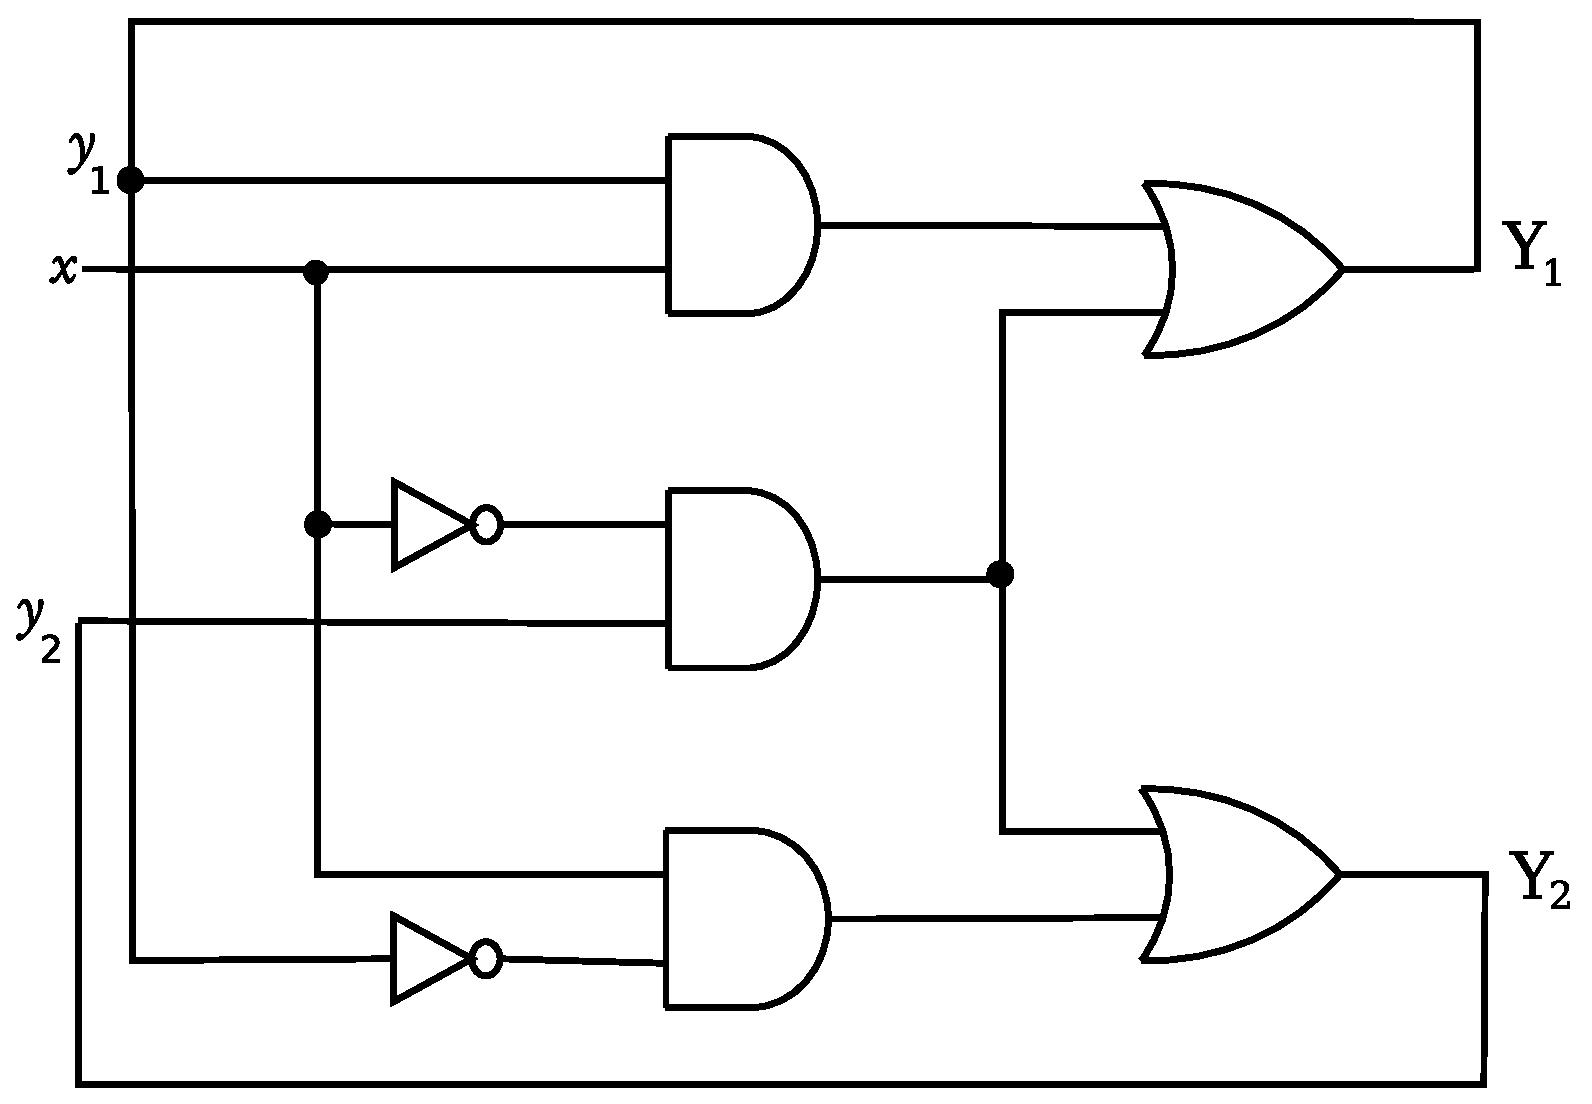
\includegraphics[scale=0.3]{src/s3/ai/09_305/digi1}
\end{center}
\Or
\item Design a serial parity generator using the asynchronous FSM technique.
\ene 

\markC
\ene

\newpage

\mainhead{D 20631}{2}
\semfour{OCTOBER 2011}
\sub{\subj}
\maxtime

\partA

\iitem State consensus theorem.
\item Simplify $f = \text{AB } + \text{BC} + \text{B}'\text{C}'.$
\item State the advantage of carry look-ahead adders.
\item Implement the following function using AND-OR realization:
  $ f = \text{ABC} + \text{A}'\text{BC}'\text{D}$.
\item Define fan-in and fan-out.

\markA
\partB

\item Implement the following function using SOP and POS forms

  $f$(A, B, C) = AB + AC + A$'$C$'$ +A$'$B$'$ + A$'$B  + AC$'$ 
\item Simplify the following function

  $f$(A, B, C, D) = $\sum m (0, 1, 2, 3, 5, 7, 8, 9, 11, 12)$
\item Design a full Adder.
\item Design a 2-bit magnitude comparator.
\item Design a 2-bit Asynchronous counter using JK flip flops.
\item Explain the basic principle of partitioning procedure.

\markB
\partCo

\item \iitem The Hamming Code 101101101 is received. Correct it if any errors. There are four parity bits
  and odd parity is used.

\newpage \again

\Or
\item Simplify the following function using Quine Mc Cluskey method

  $f$(A, B, C, D, E) = $\sum m (0, 1, 2, 3, 5, 7, 9, 12, 15, 17, 21, 25, 27, 29, 30, 31)$
\ene

\item \iitem Design a BCD adder.
\Or
\item What is a race around condition? How it is avoided in Master Slave JK flip flop? Explain.
\ene

\item \iitem Design a 4-bit universal shifter and explain its operation.
\Or
\item Draw the circuit schematic of a 2-input TTL NAND gate and explain its operation.
\ene

\item \iitem  Draw a sequential circuit for the state diagram shown in figure. Use state assignment rules
  for assigning states.

\begin{center}
  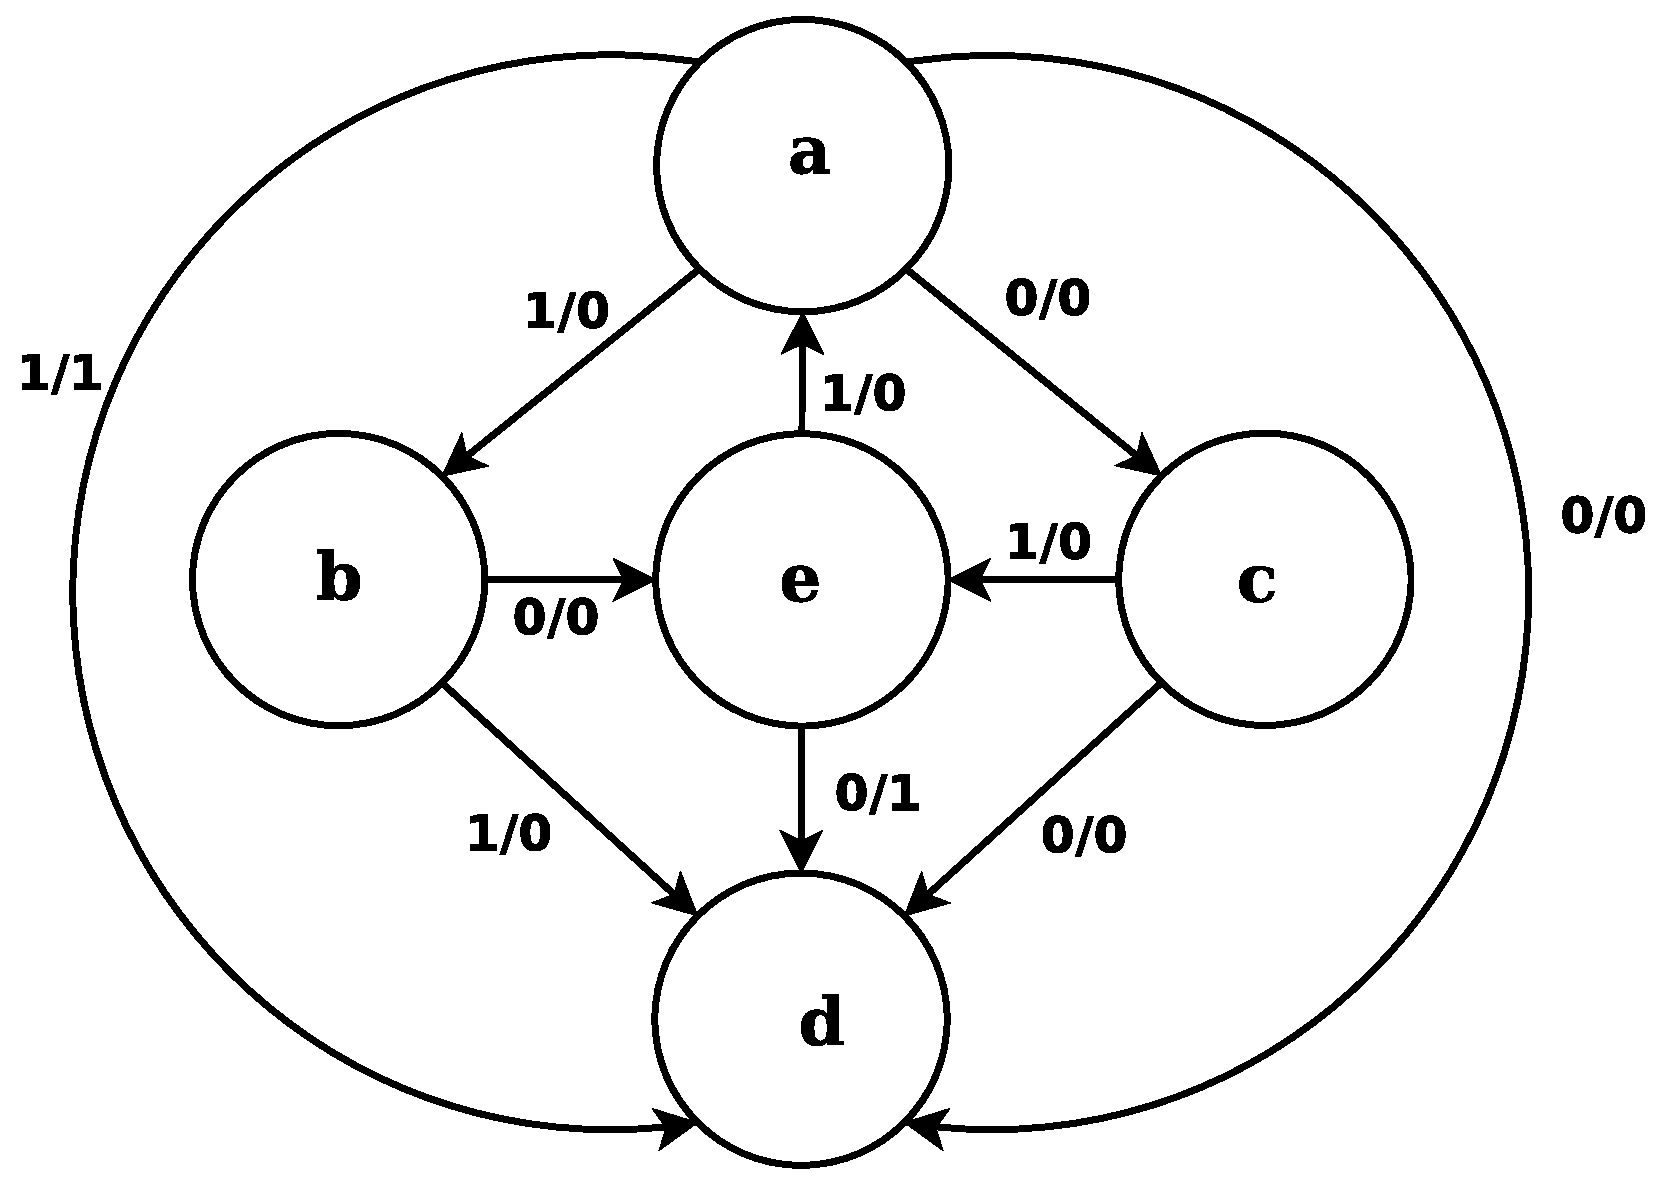
\includegraphics[scale=0.25]{src/s3/ai/09_305/digi2}
\end{center}
\item Design a sequence recogniser to detect the sequence 1011.
\ene \ene

\newpage

\mainhead{10053}{2}
\semthree{DECEMBER 2010}
\sub{\subj}
\maxtime

\partA

\iitem Convert binary number 11011.1101 to its decimal equivalent.
\item Express -54 in 2's complement form.
\item Determine the minimum number of gates required to implement
  the boolean function (AB + C) using only 2-input NOR gates.
\item What do you mean by propagation delay?
\item Draw te circuit diagram of a CMOS NAND gate.

\markA
\partB

\item Reduce boolean expression ABC + AB$\bar{\text{C}}$ + A$\bar{\text{B}}$C + $\bar{\text{A}}$BC.
\item Develop a circuit for the given expression for (A + C)($\bar{\text{B}}$ + D) using NAND gates.
\item Convert SR flipflop to JK flipflop.
\item Design a combinational logic circuit which will compare two 4 bit numbers A and B
  and produce a high output, if A$>$B and zero if A$<$B.
\item Design a circuit that will produce a PWM output with 25\% duty cycle and frequency of 
  1 KHz.
\item Design a counter that goes through the states 0, 1, 2, 4, 0 using D flipflop.

\markB
\partCo

\item \iitem Simplify the following boolean function using Quine-Mc Cluskey method.

  $f$(A, B, C, D) = $\sum m(0, 2, 3, 6, 7, 8, 10, 12, 13)$

\newpage \again

\Or
\item Reduce the following function using Karnaugh map technique and implement using
  basic gates $f$(A, B, C, D) $= \bar{\text{A}}\bar{\text{B}}$D + AB$\bar{\text{C}}\bar{\text{D}}$
  + $\bar{\text{A}}$BD + ABC$\bar{\text{D}}$.
\ene

\item \iitem Implement the following Boolean function using 4:1 multiplexer.

  $f$(A, B, C, D) = $\sum m(0, 1, 2, 4, 6, 9, 12, 14)$
\Or
\item Implement binary to BCD converter using gates.
\ene

\item \iitem Design a synchronous decade counter using T-flop flop.
\Or
\item Explain with neat diagram the operation of a 4 bit serial in parallel out
  shift register.
\ene

\item \iitem Design a synchronous counter using JK-flop flop for $4 \to 6 \to 7 \to 3 \to 1 \to 4$.
\Or
\item Explain the procedure of state minimization using merger graph and merger table.
\ene

\markC
\ene
